\documentclass[a4 paper]{article}
\usepackage[inner=2.0cm,outer=2.0cm,top=2.5cm,bottom=2.5cm]{geometry}
\usepackage{setspace}
\usepackage[ruled]{algorithm2e}
\usepackage[rgb]{xcolor}
\usepackage{verbatim}
\usepackage{subcaption}
\usepackage{amsgen,amsmath,amstext,amsbsy,amsopn,tikz,amssymb}
\usepackage{fancyhdr}
\usepackage[colorlinks=true, urlcolor=blue,  linkcolor=blue, citecolor=blue]{hyperref}
\usepackage[colorinlistoftodos]{todonotes}
\usepackage{rotating}
\usepackage{booktabs}
\newcommand{\ra}[1]{\renewcommand{\arraystretch}{#1}}
\usepackage{pythonhighlight}


\newtheorem{thm}{Theorem}[section]
\newtheorem{prop}[thm]{Proposition}
\newtheorem{lem}[thm]{Lemma}
\newtheorem{cor}[thm]{Corollary}
\newtheorem{defn}[thm]{Definition}
\newtheorem{rem}[thm]{Remark}
\numberwithin{equation}{section}

\newcommand{\homework}[6]{
	\pagestyle{myheadings}
	\thispagestyle{plain}
	\newpage
	\setcounter{page}{1}
	\noindent
	\begin{center}
		\framebox{
			\vbox{\vspace{2mm}
				\hbox to 6.28in { {\bf MATH 118:~Statistics and Probability \hfill {\small (#2)}} }
				\vspace{6mm}
				\hbox to 6.28in { {\Large \hfill #1  \hfill} }
				\vspace{6mm}
				\hbox to 6.28in { {\it Instructor: {\rm #3} \hfill Name: {\rm #5} \hfill Student Id: {\rm #6}} \hfill}
				\hbox to 6.28in { {\it Assistant: #4  \hfill #6}}
				\vspace{2mm}}
		}
	\end{center}
	\markboth{#5 -- #1}{#5 -- #1}
	\vspace*{4mm}
}

\newcommand{\problem}[2]{~\\\fbox{\textbf{Problem #1}}\hfill (#2 points)\newline\newline}
\newcommand{\subproblem}[1]{~\newline\textbf{(#1)}}
\newcommand{\D}{\mathcal{D}}
\newcommand{\Hy}{\mathcal{H}}
\newcommand{\VS}{\textrm{VS}}
\newcommand{\solution}{~\newline\textbf{\textit{(Solution)}} }

\newcommand{\bbF}{\mathbb{F}}
\newcommand{\bbX}{\mathbb{X}}
\newcommand{\bI}{\mathbf{I}}
\newcommand{\bX}{\mathbf{X}}
\newcommand{\bY}{\mathbf{Y}}
\newcommand{\bepsilon}{\boldsymbol{\epsilon}}
\newcommand{\balpha}{\boldsymbol{\alpha}}
\newcommand{\bbeta}{\boldsymbol{\beta}}
\newcommand{\0}{\mathbf{0}}


\begin{document}
	\homework{Homework \#2}{Due: 07/06/21}{Dr. Zafeirakis Zafeirakopoulos}{Gizem S\"ung\"u}{}{}
	\textbf{Course Policy}: Read all the instructions below carefully before you start working on the assignment, and before you make a submission.
	\begin{itemize}
		\item It is not a group homework. Do not share your answers to anyone in any circumstance. Any cheating means at least -100 for both sides. 
		\item Do not take any information from Internet.
		\item No late homework will be accepted. 
		\item For any questions about the homework, send an email to gizemsungu@gtu.edu.tr.
		\item Submit your homework (both your latex and pdf files in a zip file) into the course page of Moodle.
		\item Save your latex, pdf and zip files as "Name\_Surname\_StudentId".\{tex, pdf, zip\}.
		\item The answer which has only calculations without any formula and any explanation will get zero. 
		\item The deadline of the homework is 07/06/20 23:55.
		\item I strongly suggest you to write your homework on \LaTeX. However, hand-written paper is still accepted \textbf{IFF} your hand writing is \textbf{clear and understandable to read}, and the paper is well-organized. Otherwise, I cannot grade your homework.
		\item You do not need to write your Student Id on the page above. I am checking your ID from the file name.
	\end{itemize}
	
	\problem{1:}{10+10+10+10+10+10+40 = 100}
	\textbf{WARNING:} Please show your OWN work. Any cheating can be easily detected and will not be graded.
	\newline
	\newline
	For the question, please follow the file called manufacturing\_defects.txt while reading the text below.\\
	\newline
	In each year from 2000 to 2019, the number of manufacturing defects in auto manufacturers were counted. The data was collected from 14 different auto manufactory companies. The numbers of defects for the companies are indicated in 14 columns following the year column. Assume that the number of manufacturing defects per auto company per year is a random variable having a Poisson($\lambda$) and that the number of defects in different companies or in different years are independent.\\
	(Note: You should implement a code for your calculations for each following subproblem. You are free to use any programming languages (Python, R, C, C++, Java) and their related library.)
	
	\subproblem{a} Give a table how many cases occur for all companies between 2000 and 2019 for each number of defects (\# of Defects).\\
	Hint: When you check the file you will see: \# of Defects = \{0, 1, 2, 3, 4\}.
	\begin{table}[htb!]
		\centering
		\begin{tabular}{c|c}
			\begin{tabular}[c]{@{}c@{}}\textbackslash{}\# of\\Defects\end{tabular} & \begin{tabular}[c]{@{}c@{}}\textbackslash{}\# of cases\\in all company \\between the years\end{tabular}  \\ 
			\hline
			0                                                                      &  144                                                                                                         \\
			1                                                                      &     91                                                                                                     \\
			2                                                                      &       32                                                                                                   \\
			3                                                          & 11
			\\
			4                                                                      &     2                                                                                                   
		\end{tabular}
		
		\caption{Actual cases}
		\label{tab1}
	\end{table}
	
	\subproblem{b} Estimate $\lambda$ from the given data. \\ $\lambda = $ 0.7
	\subproblem{c} Update Table \ref{tab1} in Table \ref{tab2} with Poisson predicted cases with the estimated $\lambda$.\\
	\begin{table}[htb!]
		\centering
		\begin{tabular}{c|c|c}
			\begin{tabular}[c]{@{}c@{}}\textbackslash{}\# of\\Defects\end{tabular} & \begin{tabular}[c]{@{}c@{}}\textbackslash{}\# of cases\\in all companies\\between the years\end{tabular} & \begin{tabular}[c]{@{}c@{}}Predicted \textbackslash{}\# of cases\\in all companies\\between the years\end{tabular}  \\ 
			\hline
			0                                                                      &              144                                                                                            &       139                                                                                                              \\
			1                                                                      &      91                                                                                                    &    97                                                                                                                 \\
			2                                                                      &               32                                                                                           &       34                                                                                                              \\
			3                                                                      &            11                                                                                              &    7
			\\
			4                                                                      &        2                                                                                                  & 1                                                                                                                 
		\end{tabular}
		\caption{Actual vs. Predicted Cases}
		\label{tab2}
	\end{table}
	\subproblem{d} Draw a barplot for the actual cases (Table \ref{tab2} in column 2) and the predicted cases (Table \ref{tab2} column 3) with respect to \# of defecrs. You should put the figure.\\
    	
    \begin{figure*}[h!]
    	\begin{subfigure}[h]{1\textwidth}
    		\centering
    		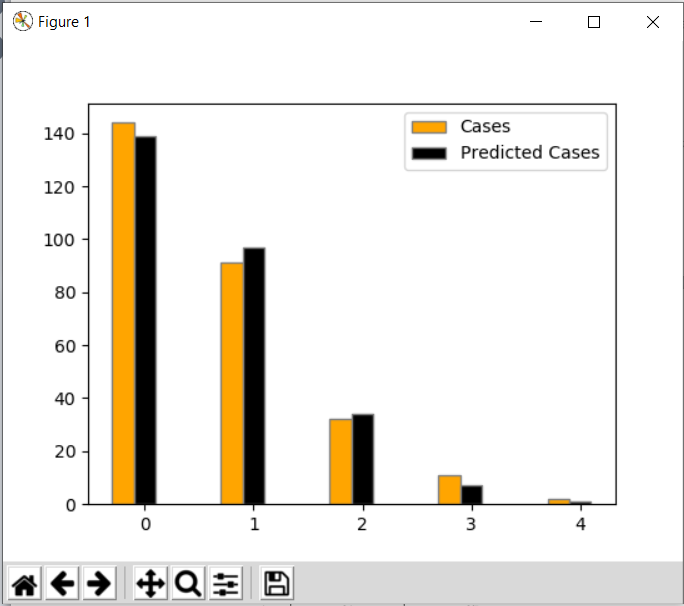
\includegraphics[height=2.8in]{barplot.png}
    		\caption{The barplot for PART D}
    	\end{subfigure}
    \end{figure*}
	
	
	\subproblem{e} According to the barplot in (c), does the poisson distribution fit the data well? Compare the values of the actual cases and the values of the poisson predicted cases, and write your opinions about performance of the distribution.\\
	
	
    I think yes, the data fits well. it is really close. For example when I compare the data for 0, compare 144 with 139, 139/144*100 means 96.52 so it means there \%96.5 similarity between the oredicted data from poisson distribution and real data. Also other cases differecy is really small to when we compare them like it seen from barplot graphic. But when the data value shrinks the difference percent get increase. For example for case 4, real case is 2 and predicted cases is 1. It is \%50 difference but when we look it as difference of numbers, it is really close to each other. So I think the performance of this poisson distrubition is really well.
    

	\newpage
	\subproblem{f} According to your estimations above, write your opinions considering your barplot and Table \ref{tab2}. Which company do you prefer to buy a car? Why?\\
	
	To find out which company is best we need to look the manufacturing\_defects file or the console output. Like it seen in console output, I would prefer to buy car from last comapny(14th). Because when I check I didn't see any 3 cases in 1 year  or any 4 cases in 1 year. I think that's really good. Also when I look to barplot I saw 0 cases are the most, 1 cases are seconder and 2 cases are third. Even the 3 case in one year and 4 case in one year is really small like it seen in data, I think if none, it's better. So I would prefer the last company because of no 3 or 4 cases in one year.
	
	\subproblem{g} Paste your code that you implemented for the subproblems above. Do not forget to write comments on your code.\\
	Example:\\
	\begin{itemize}
		\item The common code block for all subproblems\\
    		
		Paste here. Your code should read the file and compute other things which the following subproblems need.
            \begin{python}[frame=single]
            /** Reading infos in manufacturing_defects.txt */
    public void readFile(String fileName) {
        String readedLine; 

        try{
            BufferedReader bufferRead = new BufferedReader( new FileReader(fileName) );
            /** Reading all lines one by one. */
            for(int i=0; ( readedLine = bufferRead.readLine() ) != null && !readedLine.equals("\n") ; i++){
                /** Creating a list to hold the current line elements that seperated by (tab) */
                List<String> tempList = new ArrayList<String>();
                /** Splitting by tab character */
                tempList = Arrays.asList( readedLine.split("\\t") );
                //System.out.println( tempList.toString() );
                if(tempList.size() > 1){ /** if line contains a empty character, dont enter the block. */
                    /** Creating a integer list to put all splitted string elements */
                    List<Integer> intList = new ArrayList<Integer>();
                    tempList.forEach(item -> intList.add(Integer.valueOf(item) ) );
                    /** Allocate memory */
                    myList.add( new ArrayList<Integer>() );
                    /** Adding all elements to list. */
                    for(int j=0; j<intList.size(); j++){
                        myList.get(i).add( intList.get(j) );
                    }
                }
            }
            bufferRead.close(); /** Closing reader to prevent source leaks. */
        }  //End of try
        catch (IOException e) {
            System.out.println("File reading error. Check permissions and file.");
            e.printStackTrace();
        }   //End of catch.

        /** Creating memory location for toWrite ArrayList. (They will be written to temp file.) */
        for(int i=0; i<=4; i++)
            toWrite.add( new ArrayList<String>() );
        

    }
            \end{python}
            
        \newpage
		\item The code block for (a)\\
		Paste here. Your code should compute the values in Table \ref{tab1} column 2.
		\begin{python}[frame=single]
    		public int getNumberOfDefects(int whichCase){
            int total = 0;
            for(int row=0; row<myList.size(); row++){
                for(int column=2; column<myList.get(column).size(); column++){ //Starting from column 2 because column0 and 1 doesn't show case.
                    if(whichCase == myList.get(row).get(column))
                        total++;
                }
            }
            toWrite.get(whichCase).add( Integer.toString(whichCase) );
            toWrite.get(whichCase).add( Integer.toString(total) ); // writing cases to file as integer.
            return total;
        }
		\end{python}
		
		\item The code block for (b)\\
		Paste here. Your code should compute $\lambda$.
		\begin{python}[frame=single]
		    public float findRatePeriod(boolean printData){
        howManyTimesChecked = 0;
        int totalEvents = 0;
        for(int row=0; row<myList.size(); row++)
            for(int column=2; column<myList.get(column).size(); column++){ //Starting from column 2 because column0 and 1 doesnt show case.
                totalEvents += myList.get(row).get(column);
                howManyTimesChecked++;
            }
        
        float lambda = (float)totalEvents/howManyTimesChecked; /** events/time */
        if(printData == true)
            System.out.println("Total " + totalEvents + " events and " + howManyTimesChecked + " times, So mean(rate) =  $\lambda$ is " + lambda);
        return lambda;
    }
		\end{python}
		
		\item The code block for (c)\\
		Paste here. Your code should compute the values in Table \ref{tab2} column 3. 
		\begin{python}[frame=single]
    		    public double getPredictedCases(int whichCase){
            double result = 0, probability = 0;
            //false in parameter is to not printing data.
            double expLambda = Math.exp( -1 * findRatePeriod(false) ); // exp means e^(findRatePeriod) number from java.lang
            double lambdaToK = Math.pow( findRatePeriod(false) , whichCase);
            //Formula is -> $\lambda$^k * e^(- $\lambda$) / k!
    
            probability = expLambda * lambdaToK / factorial(whichCase);
            result = probability * howManyTimesChecked; //To find number of cases.
            // System.out.printf("Probability is %.2g | predicted cases is probability*timesChecked = %.2g", result, result*howManyTimesChecked);
    
            toWrite.get(whichCase).add( Integer.toString((int)result) ); // writing predicted cases to file as integer.
            return result;
        }
		\end{python}
		
		\newpage
		\item The code block for (d)\\
		Paste here. Your code should draw the barplot.
		\begin{python}[frame=single]
            import numpy as np
            import matplotlib.pyplot as plt
            
            
            with open('mat118_1801042656_hw2/temp.txt', 'r') as readingFile: # r emans read.
                # Reading line by line in while loop
                cases = []   #name of cases
                bar1 = []    #bar for cases
                bar2 = []    #bar for predicted cases
                line = readingFile.readline()  #reading first line
                while line != '':  # Until end of file.
                    print(line, end='')
                    split_string = line.split("\t") #File was splitted by tab character.
                    cases.append( split_string[0] )
                    bar1.append(  int(split_string[1]) ) #writing as int
                    bar2.append(  int(split_string[2]) ) #writing as int
                    line = readingFile.readline() #reading next line in file.
            
            # Bar positions in x axis.
            r1 = np.arange(len(bar1))   #getting length of bar1 for next bar.
            r2 = [x + 0.2 for x in r1]
            
            plt.bar(r1, bar1, width = 0.2, color = 'orange', edgecolor = 'gray', capsize=10, label='Cases')          #bar1
            plt.bar(r2, bar2, width = 0.2, color = 'black', edgecolor = 'gray', capsize=10, label='Predicted Cases') #bar2
            
            # general layout
            plt.xticks( [i + 0.2 for i in range(len(bar1))], cases) # writing cases in graphic with 0.2 distance between bars.
            plt.legend() # showing names in rectangle box.
            plt.show()   # Show graphic
		\end{python}
		
	\end{itemize}
	
	
	
	
\end{document} 


